\documentclass[aps,pra,10pt,superscriptaddress,notitlepage]{revtex4-2}
%\documentclass[a4paper,10pt,twocolumn,DIV16]{scrartcl} 

\usepackage[T1]{fontenc} %256 bit font encoding
\usepackage[english]{babel} %english language
%\usepackage{uniinput} %allows for unicode math
\usepackage[utf8]{inputenc}


\usepackage[table,usenames,dvipsnames]{xcolor}
\usepackage{hyperref}
\PassOptionsToPackage{linktocpage}{hyperref} %link numbers in TOC for arxiv

\hypersetup{
  hypertexnames=false,
  colorlinks   = true, %Colours links instead of ugly boxes
  urlcolor     = magenta, %Colour for external hyperlinks
  linkcolor    = blue, %Colour of internal links
  citecolor   = green %Colour of citations
}
\usepackage{bookmark} %to fix the pdfbookmarks

\usepackage{graphicx}
\usepackage{amsthm} % thm environments
\usepackage{amssymb}
\usepackage{amsmath,mathtools}
\usepackage{dsfont}
\usepackage[vcentermath]{youngtab}
\usepackage{comment}
\usepackage{paralist}
\usepackage{booktabs}
\usepackage{booktabs}
\usepackage{float}
\usepackage{tikz}

% package to open file containing variables
\usepackage{datatool, filecontents}
\DTLsetseparator{,}

% import data
\DTLloaddb[noheader, keys={thekey,thevalue}]{latex_vars}{report/latex_vars.dat}
\newcommand{\var}[1]{\DTLfetch{latex_vars}{thekey}{#1}{thevalue}}

\graphicspath{{mGST_results/}} %Setting the graphicspath
\makeatletter
\def\input@path{{mGST_results/}}
\makeatother



\newcommand{\tocite}[1]{{\color{blue}{[{\bf CITE:}#1]}}}
\newcommand{\comm}[1]{{\color{red}{[{\bf Comment:}#1]}}}

\newcommand{\m}[1]{\mathcal #1}
\newcommand{\ii}{\mathds{1}}


%%% =========================================================================
\begin{document}%%% =========================================================
%%% =========================================================================

\title{GST Report}
\date{\today}
\maketitle
% tableofcontents

\section{Setup}
\begin{itemize}
\item Name and date of the experiment: \var{experiment_name}, \var{experiment_date}
\item Number of sequences: 200.
\item Average shots per sequence: \var{meas_samples}.
\item \textbf{Rank: \var{rK}.}
\item Number of free parameters: \var{free_params}.
\item Gate set: \\
    \begin{center}
        \{\var{gate_labels}\}
    \end{center}
\end{itemize}

\section{Error measures}

\begin{table}[h!]
\centering
\caption{Gate quality measures}
\begin{tabular}{c|c|c|c|c|c}
\toprule
 & Average gate Fidelity & Diamond distance \\
\midrule
Idle-short & 0.9997 & 0.0430 \\
Idle-long & 0.9988 & 0.0845 \\
Rx(pi) & 0.9993 & 0.0664 \\
Ry(pi) & 0.9990 & 0.0768 \\
Rx(pi/2) & 0.9979 & 0.1132 \\
Ry(pi/2) & 0.9991 & 0.0753 \\
\bottomrule
\end{tabular}
\end{table}

\begin{table}[h!]
\centering
\caption{State and measurement quality measures}
\begin{tabular}{c|c|c|c|c|c}
\toprule
 & Final cost & Mean TVD: estimate - data & Mean TVD: target - data & POVM - diamond dist. & State - trace dist. \\
\midrule
 & 0.0031 & 0.0443 & 0.0609 & 0.1598 & 0.0160 \\
\bottomrule
\end{tabular}
\end{table}


\IfFileExists{./mGST_results/bloch_rotation.tex}{\input{mGST_results/bloch_rotation.tex}}{}
\IfFileExists{./mGST_results/bloch_rotation_axes_coeffs.tex}{\begin{table}[h!]
\centering
\caption{Normalized rotation axes coefficient.}
\begin{tabular}{c|*{6}{c}}
\toprule
 & Idle-short & Idle-long & Rx(pi) & Ry(pi) & Rx(pi/2) & Ry(pi/2) \\
\midrule
$\alpha/\pi$ & 1.986 & 1.973 & 0.992 & 0.987 & 0.486 & 0.490 \\
$n_{X}$ & 0.111 & 0.170 & -1.000 & 0.029 & -0.997 & -0.038 \\
$n_{Y}$ & 0.726 & 0.652 & -0.016 & -0.999 & 0.054 & -0.999 \\
$n_{Z}$ & -0.679 & -0.738 & 0.026 & -0.014 & -0.051 & 0.031 \\
\bottomrule
\end{tabular}
\end{table}
}{}

\newpage
\section{Gate and SPAM plots}

\foreach \x in {0,1,2,3,4,5}
{
\begin{figure*}[!ht] 
    \centering
    \includegraphics[scale=.8]{ppG\x.pdf}
    \caption{Process matrix in the Pauli basis with entries in $[-1,1]$. Left side: GST reconstruction, center: ideal gate, right side: error channel (ideally the identity).}
\end{figure*}
}

% \begin{figure*}[!ht] 
%     \centering
%     \includegraphics{spam_errs_pp.pdf}
%   \caption{Left column: state and measurement in Pauli basis, right column: magnified errors to target.}
% \end{figure*}

\begin{figure*}[!ht] 
    \centering
    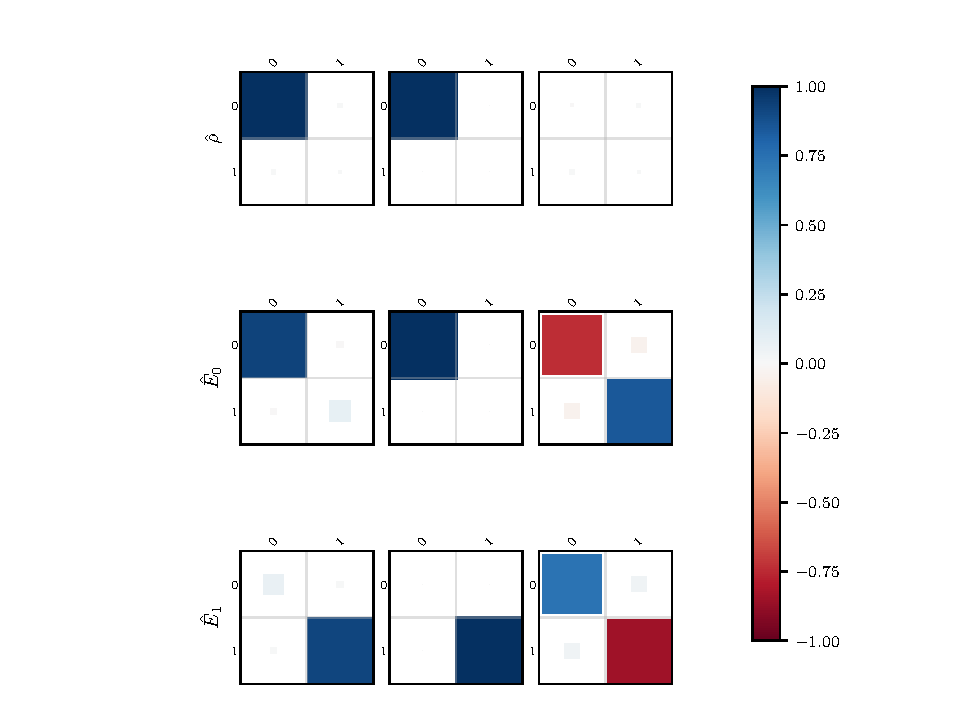
\includegraphics{spam_errs_std_real.pdf}
  \caption{Left column: real part of state and measurement in standard basis, right column: magnified errors to ideal implementation $10\cdot(\hat \rho - \rho_{\mathrm{ideal}})$ and $10\cdot(\hat E_i - E_{i,\mathrm{ideal}})$.}
\end{figure*}

\begin{figure*}[!ht] 
    \centering
    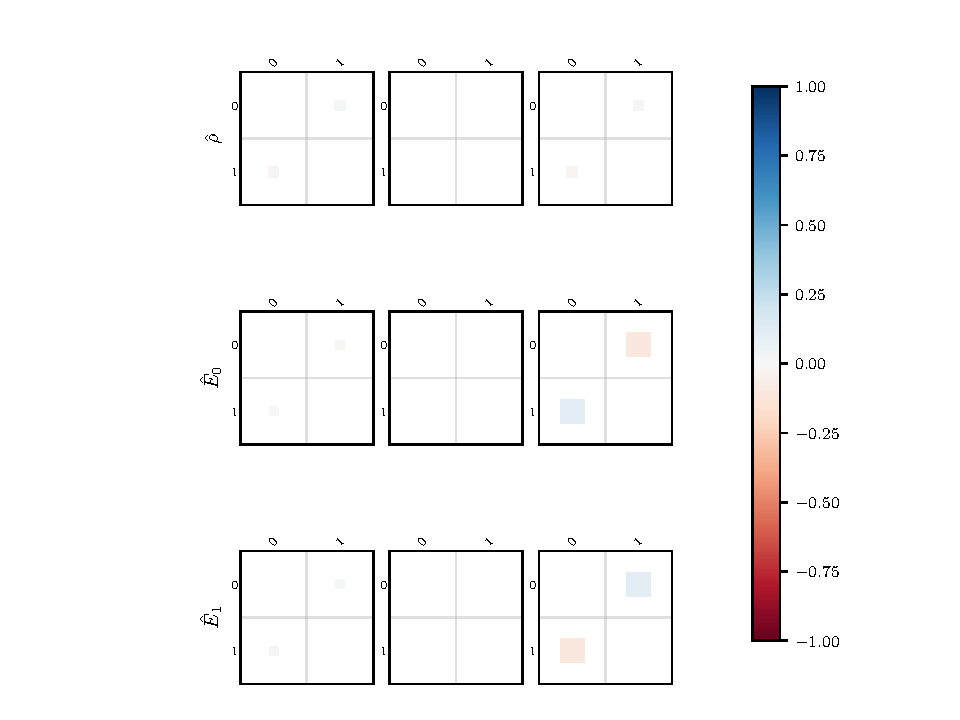
\includegraphics{spam_errs_std_imag.pdf}
  \caption{Left column: imaginary part of state and measurement in standard basis, right column: magnified errors to ideal implementation $10\cdot(\hat \rho - \rho_{\mathrm{ideal}})$ and $10\cdot(\hat E_i - E_{i,\mathrm{ideal}})$.}
\end{figure*}
%%%=============================================
%%%=============================================
\bibliographystyle{./myapsrev4-1}
\bibliography{new}
%%%=============================================


\end{document}%%%===============================
